\chapter{Security of IP Networks}
\begin{minipage}{0.6\textwidth}
%	\vspace{-0.5cm}
In IP networks, security’s main goal is to \textbf{control} who can \textbf{access} the network. In the past,
to make this possible, there were some devices called \textbf{Network Access Server (NAS)}, who’s tasks were: 
\begin{itemize}
    \item Perform \textbf{user's authN}.
    \item Perform \textbf{access control}.
    \item Eventually, provide to the user access to the IP network.
\end{itemize}
\end{minipage} 
\hspace{0.3cm}
\begin{minipage}{0.4\textwidth}
    \centering
    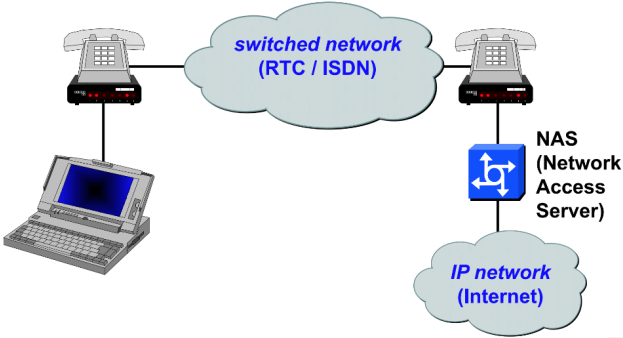
\includegraphics[width=\textwidth]{/home/lorenzo/Notes/Information System Security/images/Screenshot from 2024-12-29 17-23-09.png}
\end{minipage}
\\
\\
\noindent
\begin{minipage}{0.6\textwidth}
	\vspace{-2cm}
Nowadays, this scheme is not used anymore, as it is possible to access Internet in different
ways depending on the device. Independently of how the user decides to access the network,
user authN must always be performed before allowing any traffic from that user. 
\end{minipage} 
\hspace{0.4cm}
\begin{minipage}{0.4\textwidth}
    \vspace{0.3cm}
    \centering
    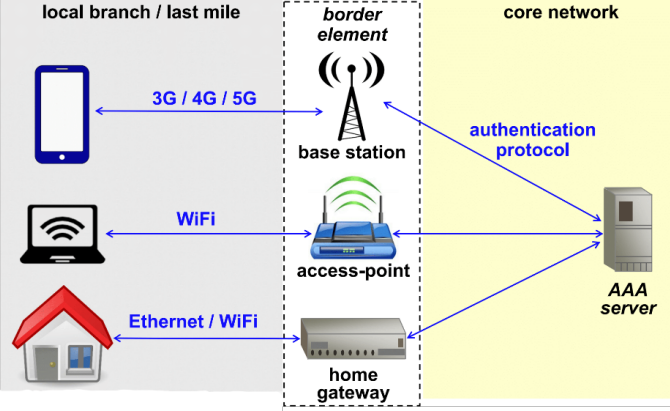
\includegraphics[width=0.9\textwidth]{/home/lorenzo/Notes/Information System Security/images/Screenshot from 2024-12-29 17-24-55.png}
\end{minipage}
\section{Authentication of PPP Channels}
There is the need to perform authN of the user \textbf{before} network transmission is enabled. Since
authN starts when someone is trying to connect, surely, the \textbf{physical} and \textbf{data layers} (L1 and L2) are already available.\\ The \textbf{Point-to-Point Protocol} (\textbf{PPP}) is a data link layer protocol (Layer 2 in the OSI model)
used for establishing direct connections between two network nodes. PPP is able to
encapsulate network packets and carry them over a point-to-point link (\(\rightarrow \)  there are many \textbf{Virtual PPP Links} going from one device to other Access Points).
\\ A \textbf{PPP link} is activated in three sequential steps:
\begin{itemize}
    \item \textbf{Link Establishment}: The devices at both ends of the link establish a connection, usually through signaling or negotiation protocols (\textbf{LCP - Link Control Protocol}).
    \item \textbf{Authentication}: If necessary (\textcolor{red}{\textbf{Optional}}), authentication takes place to verify the identity of the connecting devices, often using protocols like:
    \begin{itemize}
        \item Password Authentication Protocol (PAP)
        \item Challenge Handshake Protocol (CHAP)
        \item Extensible Authentication Protocol (EAP)
    \end{itemize} 
    \item \textbf{Network Layer Configuration}: L3 encapsulation is performed via various Network Control Protocols (NCPs), such as IP Control Protocol (IPCP) for IP packets, enabling data transfer to begin.
\end{itemize}
\newpage
\subsection{PAP (Password Authentication Protocol)}
The \textbf{oldest one}. In the case of \textbf{PAP}, the user sends username and password in \textbf{cleartext} over the PPP Link (\(\rightarrow \) authN happens \textbf{only} once the PPP Link is created, so sniffing and MITM attacks are possible).
\vspace{-0.4cm}
\begin{center}
\begin{quotebox-grey}{\textbf{PAP} uses a \textbf{2-way Handshake Protocol}:}
    \begin{enumerate}
        \item \textbf{Authenticate Request} (\textbf{Code = 1}), the peer sends to the authenticator the following packet:
        \begin{itemize}
            \item Code (8 bits) + Identifier (8 bits) + Length (16 bits)
            \item PeerID Length in bytes (8 bits) + PeerID (0-255 bytes)
            \item Password Length in bytes (8 bits) + Password (0-255 bytes)
        \end{itemize}
        \item \textbf{Authenticate Response} (\textbf{Code = 2, 3}), the authenticator sends to the peer the following packet:
        \begin{itemize}
            \item Code (8 bits) + Identifier (8 bits) + Length (16 bits), where:
            \begin{itemize}
                \item If the previous data was received correctly \(\rightarrow \) Code = 2 (ACK)
                \item Else \(\rightarrow \) Code = 3 (NAK)
            \end{itemize}
            \item Message Lenght in bytes (8 bits) + Message (0-255 bytes)
        \end{itemize}
    \end{enumerate}
\end{quotebox-grey}
\end{center}
\noindent
The Identifier \textbf{must} match between request and response. Moreover, the request or the response may be lost, so the authenticator \textbf{must} allow multiple requests from the same peer.

\subsection{CHAP (Challenge Handshake Authentication Protocol)}
\textbf{CHAP} uses a Symmetric CRA who’s response is based on the user’s password, the initial challenge is generated at the \textbf{creation} of the PPP Link (\(\rightarrow \) Sniffing attacks are not possible, but MITM attacks still are). CHAP is \textbf{safer} than PAP, so if an authenticator supports PAP and CHAP \(\rightarrow \) CHAP \textbf{must} be offered first.
\vspace{-0.4cm}
\begin{center}
\begin{quotebox-grey}{CHAP uses a \textbf{3-way Handshake Protocol}:}
    \begin{enumerate}
        \item \textbf{Challenge} (\textbf{Code = 1}), the authenticator sends to the peer the following packet:
        \begin{itemize}
            \item Code (8 bits) + Identifier (8 bits) + Length (16 bits)
            \item Challenge Size in bytes (8 bits) + Challenge (0-255 bytes)
        \end{itemize}
        \item \textbf{Response} (\textbf{Code = 2}), the peer sends to the authenticator the following packet:
        \begin{itemize}
            \item Code (8 bits) + Identifier (8 bits) + Length (16 bits)
            \item Response Size in bytes (8 bits) + Response (0-255 bytes), where:
            \[Response\ =\ MD5(Identifier\ ||\ Password\ ||\ Challenge)\]
        \end{itemize}
        \item \textbf{Result} (\textbf{Code = 3, 4}), the authenticator sends to the peer the following packet:
        \begin{itemize}
            \item Code (8 bits) + Identifier (8 bits) + Length (16 bits), where:
            \begin{itemize}
                \item If response was correct \(\rightarrow \) Code = 3
                \item Else \(\rightarrow \) Code = 4
            \end{itemize}
        \end{itemize}
    \end{enumerate}
\end{quotebox-grey}
\end{center}
\noindent
As in PAP, the Identifier \textbf{must} match between challenge and response. Moreover, the challenge or the response may be lost, so the authenticator \textbf{must} resend a \textbf{different} (nonce, random, non-invertible) challenge if no response arrives (up until the retry limit is hit).

\begin{customquote}
\vspace{-0.4cm}
\subsubsection{MS-CHAP}
\textbf{MS-CHAP} is the \textbf{Microsoft extension} of CHAP, every Windows system from Windows Vista to Win11 22H2 uses it. MS-CHAP has two official versions, v1 and v2:
\begin{itemize}
    \item \textbf{Common Traits}:
    \begin{itemize}
        \item Authenticator controlled password change.
        \item Authenticator controlled authN retry.
        \item Specific failure codes.
    \end{itemize}
    \item \textbf{v2 updates}: v2 provides \textbf{mutual authN} by piggybacking a peer challenge on the response and by adding an authenticator response on the Success packet.
\end{itemize}
\vspace{-1cm}
\begin{quotebox-red}{Beware}
    \textbf{MS-CHAPv2} should \textbf{never} be used! Since with just \(2^{56}\) operations (\(\sim\) 23 hours with DES
FPGA) we can decrypt the response \(\rightarrow \) critical security errors in the protocol.

\end{quotebox-red}
\end{customquote}

